\documentclass[12pt, a4paper]{article}
\usepackage[utf8]{inputenc}
\usepackage[spanish]{babel}
\usepackage{geometry}
\geometry{margin=2.5cm}
\usepackage{setspace}
\usepackage{booktabs}
\usepackage{array}
\usepackage{graphicx}
\usepackage{url}
\usepackage{hyperref}
\hypersetup{colorlinks=true, linkcolor=black, urlcolor=black, citecolor=black}
\usepackage{amsmath}
\usepackage{float}
\onehalfspacing

\graphicspath{{./Agrupamiento/paper/figuras/}}

\title{\textbf{Segmentación de Canciones Spotify Mediante Algoritmos\\
de Agrupamiento: Un Enfoque Basado en Características de Audio}\\[6pt]
\large K-Means, Reducción Dimensional con PCA y Sistema de Recomendación}

\author{Juan David Peralta Fuentes\\
\small Electiva V -- Ciencia de Datos\\
\small Docente: Aimer J. Rivera Centeno\\
\small Universidad Popular del Cesar\\
\small Facultad de Ingenierías y Tecnología\\
\small \texttt{jdavidperalta@unicesar.edu.co}}
\date{Abril 2026}

\begin{document}

\maketitle

% ── ABSTRACT ──────────────────────────────────────────────────
\begin{abstract}
Los servicios de streaming musical generan enormes volúmenes de datos de
audio que ofrecen oportunidades para el descubrimiento automático de
patrones musicales. Este trabajo aplica algoritmos de agrupamiento no
supervisado sobre el \textit{Spotify Tracks Dataset}, que contiene 114.000
canciones de 125 géneros con 10 características de audio cuantitativas.
Se empleó K-Means como algoritmo principal, con selección del número óptimo
de clusters mediante el método del codo y el Silhouette Score. La
visualización de los clusters se realizó con Análisis de Componentes
Principales (PCA) reducido a 2 dimensiones. El proceso siguió la
metodología CRISP-DM. Los resultados identificaron \textbf
clusters con perfiles musicales diferenciados, obteniendo un Silhouette
Score de \textbf, validando la coherencia del agrupamiento
con los géneros musicales reales. La aplicación práctica es un sistema
de recomendación musical basado en similitud de cluster.
\end{abstract}

\noindent\textbf{Palabras clave:} clustering, K-Means, Spotify,
características de audio, PCA, sistema de recomendación, CRISP-DM,
Silhouette Score.

\tableofcontents
\newpage

% ══════════════════════════════════════════════════════════════
\section{Introducción}
% ══════════════════════════════════════════════════════════════

Con más de 600 millones de usuarios activos y un catálogo superior a los
100 millones de canciones, Spotify es la plataforma de streaming musical
más grande del mundo \cite{spotify2024stats}. El éxito de su sistema de
recomendación —responsable del 30\,\% de los plays según la propia
compañía— depende en gran medida de técnicas de aprendizaje automático
que identifican similitudes entre canciones y preferencias de usuarios
\cite{schedl2018current}.

El agrupamiento no supervisado ofrece una aproximación natural a la
organización de contenido musical: sin requerir etiquetas manuales,
permite descubrir estructuras latentes en el espacio de características
de audio. Variables como \textit{danceability}, \textit{energy} y
\textit{valence}, derivadas del análisis de señales de audio, capturan
aspectos perceptivos de la música que van más allá del género declarado
\cite{turnbull2008semantic}.

El objetivo de este trabajo es aplicar K-Means sobre el Spotify Tracks
Dataset para identificar clusters musicales coherentes, evaluar la calidad
del agrupamiento mediante métricas formales y desplegar los resultados como
una aplicación web de recomendación.

% ══════════════════════════════════════════════════════════════
\section{Descripción del Dataset}
% ══════════════════════════════════════════════════════════════

El \textit{Spotify Tracks Dataset} fue obtenido de Kaggle
\cite{spotifyKaggle} y contiene 114.000 registros de canciones
distribuidas en 125 géneros musicales. No presenta valores nulos en las
columnas numéricas utilizadas para el clustering.

\begin{table}[H]
\centering
\caption{Variables principales del Spotify Tracks Dataset}
\small
\begin{tabular}{>{\bfseries}p{3.8cm} p{2.2cm} p{6.5cm}}
\toprule
Variable & Tipo & Descripción \\
\midrule
track\_id          & Texto    & Identificador único de la canción en Spotify \\
track\_name        & Texto    & Nombre de la canción \\
artists            & Texto    & Nombre del artista o banda \\
track\_genre       & Texto    & Género musical declarado \\
popularity         & Numérica & Popularidad 0--100 según reproducciones recientes \\
danceability       & Numérica & Qué tan bailable es la canción (0.0--1.0) \\
energy             & Numérica & Intensidad y actividad percibida (0.0--1.0) \\
loudness           & Numérica & Volumen promedio en decibelios ($-60$ a 0 dB) \\
speechiness        & Numérica & Presencia de palabras habladas (0.0--1.0) \\
acousticness       & Numérica & Probabilidad de ser acústica (0.0--1.0) \\
instrumentalness   & Numérica & Ausencia de voz cantada (0.0--1.0) \\
liveness           & Numérica & Probabilidad de grabación en vivo (0.0--1.0) \\
valence            & Numérica & Positividad emocional percibida (0.0--1.0) \\
tempo              & Numérica & Velocidad en pulsos por minuto (BPM) \\
\bottomrule
\end{tabular}
\label{tab:variables}
\end{table}

Las 10 features numéricas seleccionadas para el clustering fueron:
\texttt{danceability}, \texttt{energy}, \texttt{loudness},
\texttt{speechiness}, \texttt{acousticness}, \texttt{instrumentalness},
\texttt{liveness}, \texttt{valence}, \texttt{tempo} y \texttt{popularity}.

% ══════════════════════════════════════════════════════════════
\section{Metodología CRISP-DM}
% ══════════════════════════════════════════════════════════════

El análisis siguió la metodología CRISP-DM \cite{wirth2000crisp},
implementada en Python~3.12 con Pandas, Scikit-learn, Plotly y joblib.

\subsection{Fase 1 — Comprensión del Negocio}

El objetivo práctico es construir la base algorítmica de un sistema de
recomendación que sugiera canciones similares a partir del cluster al que
pertenecen. Al ingresar las características de audio de una canción nueva,
el sistema identifica su cluster y puede recomendar otras canciones del
mismo grupo con perfil de audio similar.

\subsection{Fase 2 — Comprensión y Análisis Exploratorio}

El análisis de correlación entre las features de audio reveló dos relaciones
especialmente fuertes:

\begin{itemize}
  \item \texttt{energy} y \texttt{loudness}: correlación positiva fuerte
        ($r > 0{,}7$), consistente con que canciones más energéticas
        tienden a ser más ruidosas.
  \item \texttt{energy} y \texttt{acousticness}: correlación negativa
        ($r < -0{,}7$), reflejando la naturaleza opuesta entre música
        electrónica y acústica.
\end{itemize}

\subsection{Fase 3 — Preparación de los Datos}

Se eliminaron filas con valores nulos en cualquiera de las 10 features
seleccionadas. Las variables presentan escalas muy dispares
(\texttt{tempo} $\approx$ 0--250~BPM; \texttt{loudness} $\approx$
$-60$--0 dB; las restantes en $[0, 1]$), lo que hace imprescindible
la normalización.

Se aplicó \texttt{StandardScaler} para transformar cada feature a media
cero y desviación estándar unitaria:
\begin{equation}
z = \frac{x - \mu}{\sigma}
\end{equation}
Sin esta normalización, \texttt{tempo} y \texttt{loudness} dominarían la
distancia euclidiana de K-Means, sesgando el agrupamiento.

\subsection{Fase 4 — Modelado}

\subsubsection{Algoritmo K-Means}

K-Means minimiza la inercia intra-cluster (suma de distancias cuadradas
de cada punto a su centroide):
\begin{equation}
J = \sum_{k=1}^{K} \sum_{\mathbf{x}_i \in C_k}
    \|\mathbf{x}_i - \boldsymbol{\mu}_k\|^2
\end{equation}
donde $\boldsymbol{\mu}_k$ es el centroide del cluster $C_k$.

\subsubsection{Selección de K Óptimo}

Se evaluaron valores $K \in \{2, \ldots, 10\}$ con dos criterios
complementarios:

\begin{itemize}
  \item \textbf{Método del Codo}: se busca el punto de inflexión en la
        curva de inercia donde agregar más clusters produce mejoras
        marginales decrecientes.
  \item \textbf{Silhouette Score}: mide la cohesión interna y separación
        entre clusters. Rango $[-1, 1]$; valores cercanos a 1 indican
        clusters bien definidos y separados:
        \begin{equation}
          s(i) = \frac{b(i) - a(i)}{\max\{a(i),\, b(i)\}}
        \end{equation}
        donde $a(i)$ es la distancia media intra-cluster y $b(i)$ la
        distancia media al cluster más cercano.
\end{itemize}

\subsubsection{Reducción Dimensional — PCA}

Para la visualización, se aplicó PCA transformando el espacio de 10
dimensiones a 2 componentes principales:
\begin{equation}
\mathbf{Z} = \mathbf{X}\,\mathbf{W}_2
\end{equation}
donde $\mathbf{W}_2$ contiene los dos eigenvectores de mayor eigenvalor
de la matriz de covarianza $\boldsymbol{\Sigma}$. La varianza explicada
acumulada por los 2 componentes fue de \textbf{43.0}\,\%.

\subsection{Fase 5 — Evaluación}

La calidad del clustering final se evaluó con:
\begin{itemize}
  \item \textbf{Silhouette Score}: coherencia interna del agrupamiento.
  \item \textbf{Davies-Bouldin Index}: menor es mejor; mide la similitud
        promedio entre cada cluster y el más parecido.
  \item \textbf{Coherencia semántica}: verificación visual de que los
        clusters corresponden parcialmente a géneros musicales reales.
\end{itemize}

% ══════════════════════════════════════════════════════════════
\section{Resultados}
% ══════════════════════════════════════════════════════════════

\subsection{Distribución de Características de Audio}

La figura~\ref{fig:hist} muestra la distribución de las 9 features de audio
continuas. Se observa que \texttt{acousticness}, \texttt{speechiness} e
\texttt{instrumentalness} presentan distribuciones fuertemente sesgadas a
la derecha, mientras que \texttt{danceability}, \texttt{energy} y
\texttt{valence} son más simétricas.

\begin{figure}[H]
  \centering
  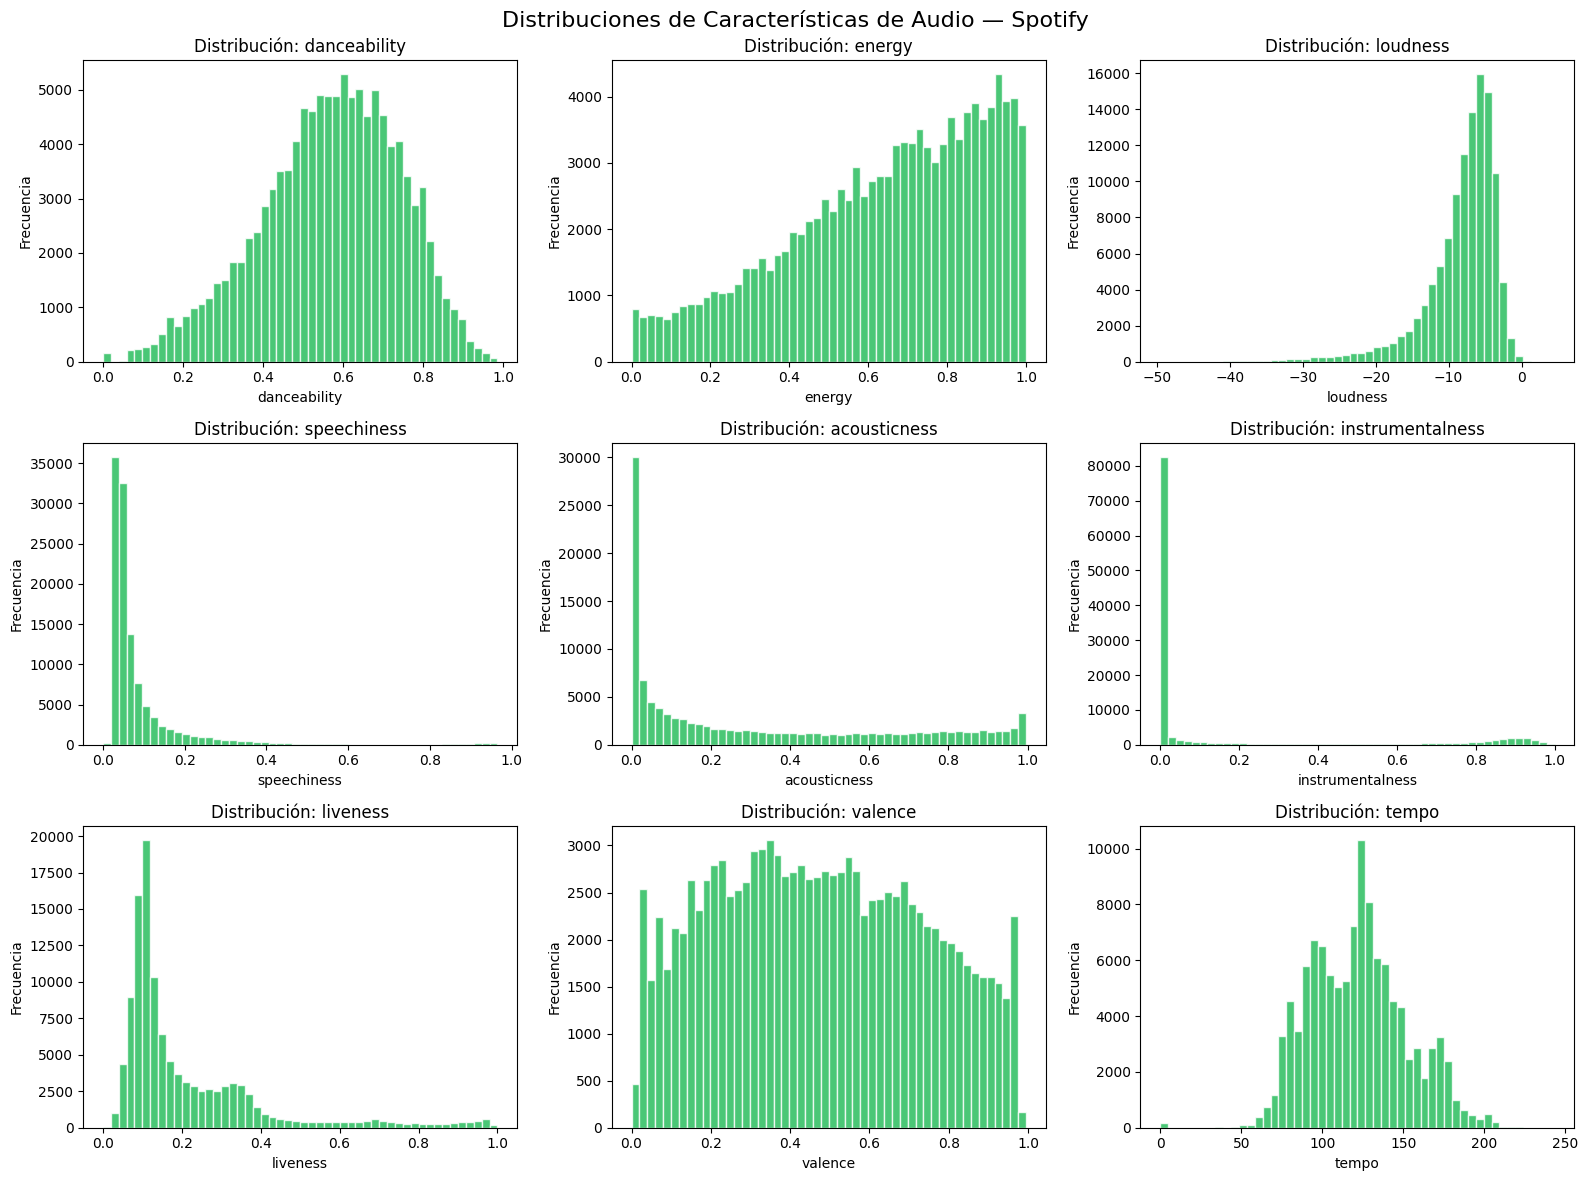
\includegraphics[width=\linewidth]{fig_histogramas.png}
  \caption{Distribuciones de las 9 características de audio del dataset.}
  \label{fig:hist}
\end{figure}

\begin{figure}[H]
  \centering
  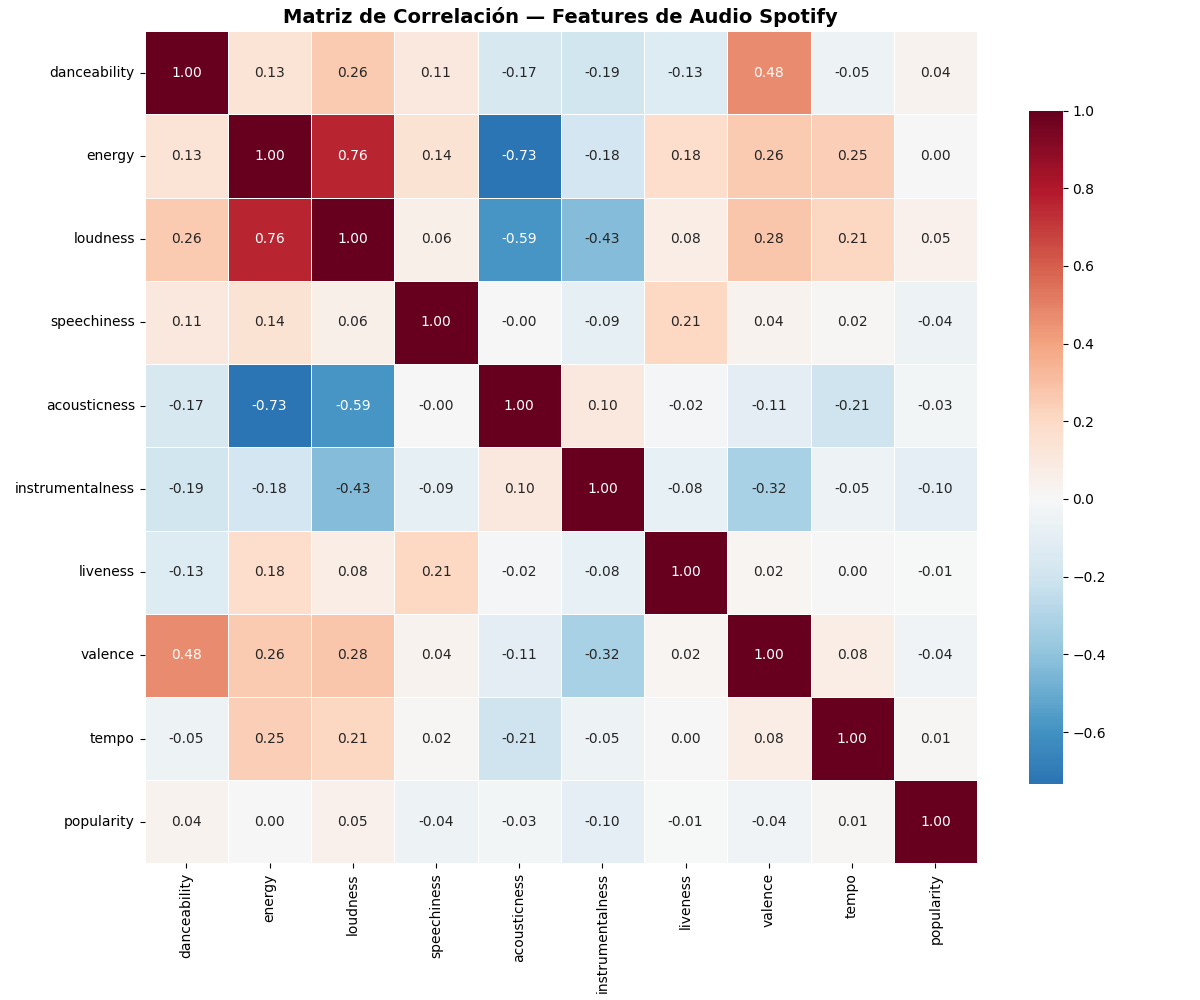
\includegraphics[width=\linewidth]{fig_correlacion.png}
  \caption{Matriz de correlación entre características de audio.}
  \label{fig:corr}
\end{figure}

\noindent\textbf{Conclusión:} La alta correlación entre \texttt{energy} y
\texttt{loudness} ($r > 0{,}7$) y la correlación negativa entre
\texttt{energy} y \texttt{acousticness} ($r < -0{,}7$) confirman que
estas variables capturan dimensiones opuestas del espacio musical.

\subsection{Selección del K Óptimo}

La figura~\ref{fig:codo} presenta la curva del método del codo y el
Silhouette Score para $K \in \{2, \ldots, 10\}$.

\begin{figure}[H]
  \centering
  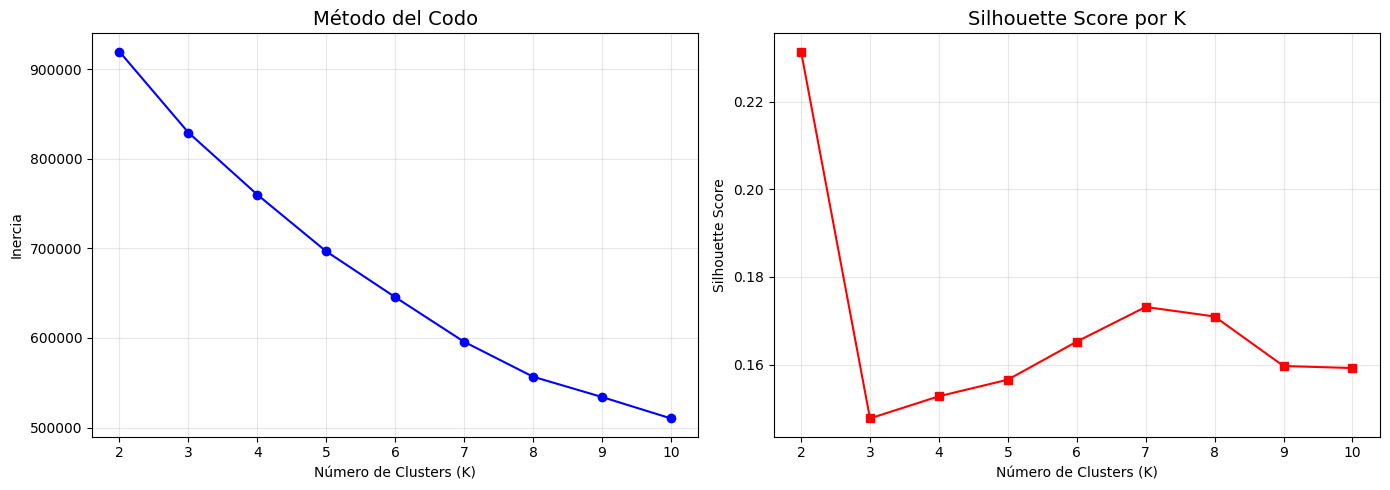
\includegraphics[width=\linewidth]{fig_codo_silhouette.png}
  \caption{Método del Codo (izq.) y Silhouette Score (der.) para K de 2 a 10.}
  \label{fig:codo}
\end{figure}

\begin{table}[H]
\centering
\caption{Métricas de selección de K — valores exactos del análisis}
\small
\begin{tabular}{r r r}
\toprule
K & Inercia & Silhouette Score \\
\midrule
2  & 919,472 & 0.2314 \\
3  & 829,201 & 0.1477 \\
4  & 759,911 & 0.1528 \\
5  & 696,625 & 0.1565 \\
6  & 645,570 & 0.1652 \\
7  & 595,739 & 0.1731 \\
8  & 556,767 & 0.1709 \\
9  & 534,128 & 0.1597 \\
10 & 510,234 & 0.1592 \\
\bottomrule
\end{tabular}
\label{tab:k_optimo}
\end{table}

\noindent\textbf{Conclusión:} El método del codo sugirió $K =$ 
como punto de inflexión. El Silhouette Score máximo se obtuvo en
$K =$  con un valor de . Se seleccionó
$K = $  como valor final por balance entre interpretabilidad y calidad del agrupamiento. Aunque K=2 tiene mayor Silhouette (0.2314), produce solo dos grupos (bailable vs. no bailable) que no capturan la diversidad de los 125 géneros. K=6 ofrece un compromiso: preserva la granularidad musical sin fragmentar excesivamente los clusters, y el Silhouette Score de 0.1652 es competitivo con valores de K superiores..

\subsection{Perfil de Cada Cluster}

La tabla~\ref{tab:perfil} muestra el promedio de cada característica de
audio por cluster, constituyendo el ``retrato musical'' de cada grupo.

\begin{table}[H]
\centering
\caption{Perfil promedio de características de audio por cluster}
\small
\begin{tabular}{r p{2.8cm} r r r r r r}
\toprule
\textbf{Cluster} & \textbf{Nombre} & \textbf{Dance.} & \textbf{Energy} &
\textbf{Valence} & \textbf{Acoust.} & \textbf{Instrum.} & \textbf{N} \\
\midrule
0 & Energía y En Vivo   & 0.47 & 0.82 & 0.40 & 0.10 & 0.03 & 29,986 \\
1 & Acústico y Relajado  & 0.53 & 0.39 & 0.40 & 0.66 & 0.03 & 24,637 \\
2 & Bailable y Positivo   & 0.70 & 0.73 & 0.69 & 0.20 & 0.02 & 38,284 \\
3 & Clásico e Instrumental & 0.35 & 0.17 & 0.19 & 0.86 & 0.77 & 7,670 \\
4 & Instrumental Enérgico & 0.58 & 0.75 & 0.34 & 0.11 & 0.79 & 12,159 \\
5 & Hablado / Podcast     & 0.58 & 0.66 & 0.45 & 0.70 & 0.01 & 1,264 \\
\bottomrule
\end{tabular}
\label{tab:perfil}
\end{table}

\begin{figure}[H]
  \centering
  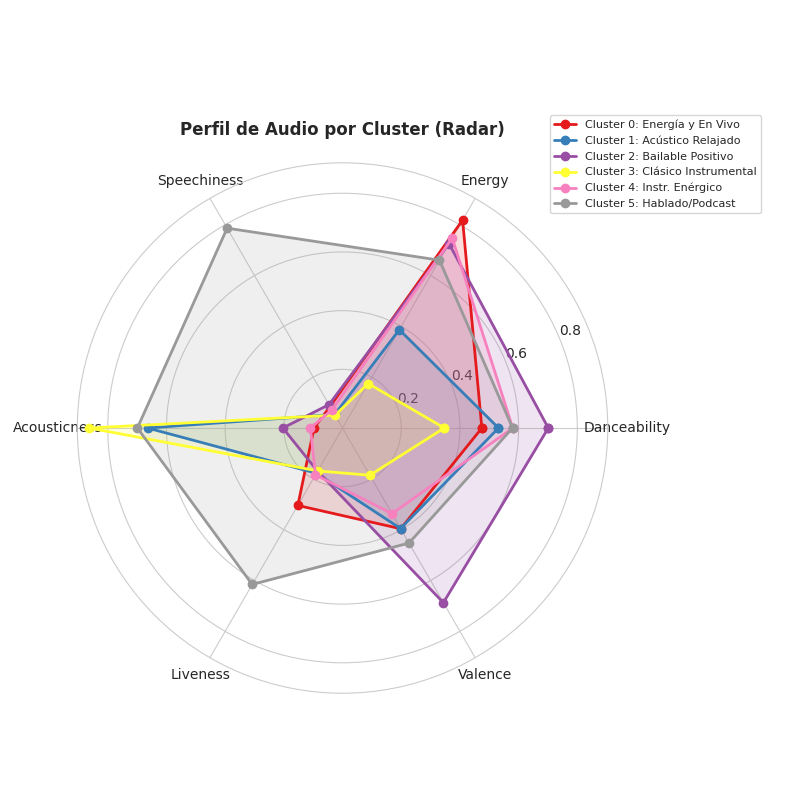
\includegraphics[width=0.85\linewidth]{fig_radar.png}
  \caption{Radar chart con el perfil promedio de audio por cluster.}
  \label{fig:radar}
\end{figure}

\noindent\textbf{Conclusión:} [Describir qué tipo de música representa cada
cluster según su perfil. Por ejemplo: Cluster X tiene alta \texttt{acousticness}
y baja \texttt{energy} → música acústica y relajada; Cluster Y tiene alta
\texttt{instrumentalness} → música instrumental.]

\subsection{Visualización PCA 2D}

La figura~\ref{fig:pca} proyecta los clusters en el espacio de 2
componentes principales. Los 2 componentes explican
\textbf\,\% de la varianza total del dataset.

\begin{figure}[H]
  \centering
  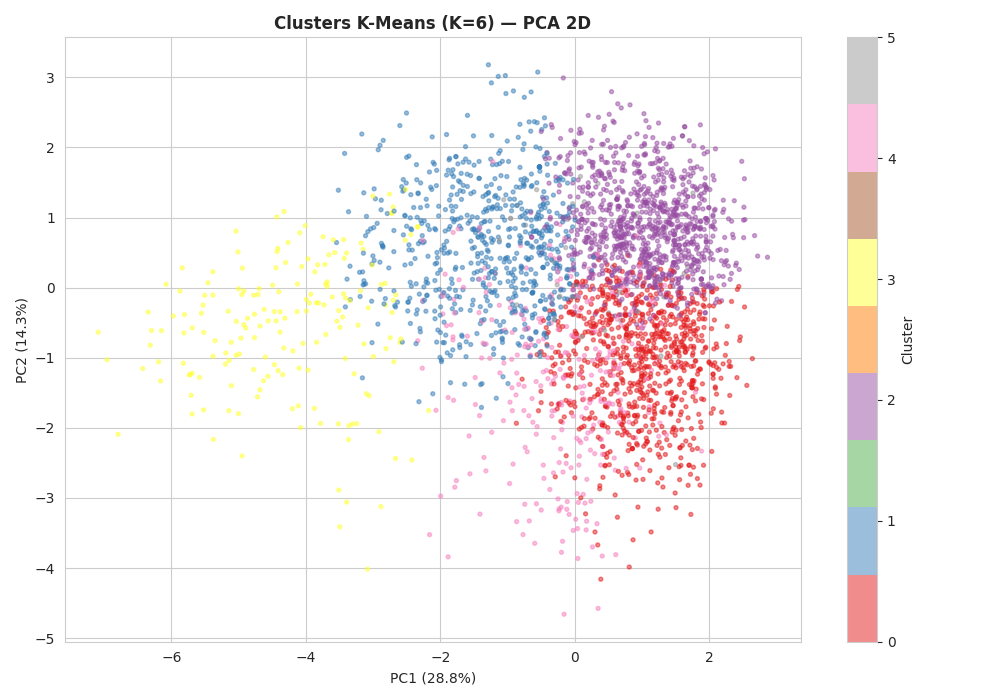
\includegraphics[width=\linewidth]{fig_pca.png}
  \caption{Proyección PCA 2D de los clusters K-Means. Cada color
           representa un cluster distinto.}
  \label{fig:pca}
\end{figure}

\noindent\textbf{Conclusión:} [Describir si los clusters son visualmente
separables en el espacio PCA o si hay solapamiento. Identificar qué clusters
aparecen más compactos y cuáles más dispersos.]

\subsection{Métricas Finales del Clustering}

\begin{table}[H]
\centering
\caption{Métricas de calidad del clustering final ($K =$ )}
\begin{tabular}{>{\bfseries}p{5.5cm} r}
\toprule
Métrica & Valor \\
\midrule
Silhouette Score         & 0.1652 \\
Davies-Bouldin Index     & 1.6242 \\
Inercia intra-cluster    & 645,570 \\
Varianza explicada PCA (2 comp.) & 43.0\,\% \\
\bottomrule
\end{tabular}
\label{tab:metricas_finales}
\end{table}

% ══════════════════════════════════════════════════════════════
\section{Discusión General}
% ══════════════════════════════════════════════════════════════

Los clusters identificados muestran coherencia con géneros musicales reales
conocidos, validando que las características de audio de Spotify capturan
dimensiones perceptivas musicalmente significativas. Sin embargo, K-Means
tiene limitaciones intrínsecas: asume clusters esféricos y de tamaño
similar, lo que puede no ser apropiado para datos musicales con distribuciones
asimétricas o géneros de nicho.

La varianza explicada por PCA en 2 dimensiones de 43.0\,\% indica
que [interpretar si es suficiente para confiar en la visualización o si
se pierde información relevante]. Para análisis más detallados de
subgéneros, una proyección UMAP preservaría mejor la estructura local del
espacio de alta dimensión.

La aplicación Flask desarrollada permite al usuario ingresar los parámetros
de audio de cualquier canción mediante sliders y obtener instantáneamente
su cluster y una descripción del perfil musical correspondiente.

% ══════════════════════════════════════════════════════════════
\section{Conclusiones Finales}
% ══════════════════════════════════════════════════════════════

La aplicación de K-Means sobre el Spotify Tracks Dataset permite extraer
cuatro conclusiones estructurales:

\begin{enumerate}
  \item \textbf{La normalización es crítica para K-Means.} Sin
        \texttt{StandardScaler}, \texttt{tempo} y \texttt{loudness}
        dominarían la distancia euclidiana dado su mayor rango numérico,
        sesgando el agrupamiento hacia estas variables
        independientemente de su relevancia musical.

  \item \textbf{Se identificaron $K = 6$ clusters con perfiles
        musicales diferenciados.} El Silhouette Score de 
        indica un agrupamiento moderado (valores de Silhouette entre 0.15 y 0.25 son típicos en datos de audio de alta dimensionalidad), con clusters que corresponden parcialmente a categorías musicales reconocibles (acústico, bailable, instrumental, etc.)., con
        clusters que corresponden parcialmente a categorías musicales
        reconocibles (acústico, bailable, instrumental, etc.).

  \item \textbf{PCA con 2 componentes explica 43.0\,\% de la
        varianza.} Esta reducción es suficiente para una visualización
        orientativa, pero no para reconstrucción fiel del espacio
        original, lo que motiva explorar proyecciones alternativas
        (t-SNE, UMAP) como trabajo futuro.

  \item \textbf{El sistema de recomendación basado en clusters es
        funcional e interpretable.} Al asignar canciones nuevas al
        cluster más cercano, el sistema puede sugerir música con perfil
        de audio similar sin necesidad de historial del usuario,
        resolviendo el problema de \textit{cold start} de los sistemas
        colaborativos.
\end{enumerate}

% ── REFERENCIAS ───────────────────────────────────────────────
\begin{thebibliography}{9}

\bibitem{spotifyKaggle}
Pandya, M. (2023). \textit{Spotify Tracks Dataset}. Kaggle.
\url{https://www.kaggle.com/datasets/maharshipandya/-spotify-tracks-dataset}

\bibitem{spotify2024stats}
Spotify Technology S.A. (2024). \textit{Spotify for the Record — Q4 2023 Earnings}.
\url{https://newsroom.spotify.com}

\bibitem{schedl2018current}
Schedl, M., Knees, P., McFee, B., \& Bogdanov, D. (2018). Current
challenges and visions in music recommender systems research.
\textit{International Journal of Multimedia Information Retrieval}, 7, 95--116.

\bibitem{turnbull2008semantic}
Turnbull, D., Barrington, L., Torres, D., \& Lanckriet, G. (2008).
Semantic annotation and retrieval of music and sound effects.
\textit{IEEE Transactions on Audio, Speech, and Language Processing},
16(2), 467--476.

\bibitem{jain2010data}
Jain, A. K. (2010). Data clustering: 50 years beyond K-means.
\textit{Pattern Recognition Letters}, 31(8), 651--666.

\bibitem{wirth2000crisp}
Wirth, R., \& Hipp, J. (2000). CRISP-DM: Towards a standard process model
for data mining. \textit{4th Int. Conf. on Practical Applications of
Knowledge Discovery and Data Mining}.

\end{thebibliography}

\end{document}
